\subsubsection{Creació de les caselles de selecció per cada continent}

\paragraph{}
Intentar crear la secció de caselles de selecció (checkboxes), de forma manual, en el HTML, hauria estat una bogeria. No només per l’elevada quantitat de feina manual, sinó també per la poca impracticabilitat d’aquesta. La creació d'aquestes seccions, s'ha realitzat mitjançant la creació d’HTML dinàmic de Mustache.

El servidor, mitjançant Mustache, utilitza la informació continguda en el fitxer \emph{countryParameters.js}, per crear un procés iteratiu que genera totes les caselles necessàries per a cada continent.

Per exemple, pel continent nord-americà, s'utilitza el següent bloc de codi. Recordem que les etiquetes \emph{\{\{\#northAmerica\}\}} i \emph{\{\{/northAmerica\}\}}, indiquen que es vol replicar el HTML situat entre elles per cada element del vector \emph{northAmerica}.

\begin{lstlisting}[style=rawOwn,caption={Caselles de selecció creades mitjançant Mustache}]
{{#northAmerica}}
    <div class=`col-md-3 col-sm-6 col-xs-12'>
        <label class=`checkbox-inline'>
        <input type=`checkbox' id=`{{code}}' ... > {{name}}
    </label>
<div>
{{/northAmerica}}
\end{lstlisting}

D'aquesta forma, per cada país contingut en l’objecte \emph{northAmercia}, es representa el nom del país \emph{(\{\{name\}\})}  i s'emmagatzema el codi d'aquest en el camp ID \emph{(\{\{code\}\})}, per tal de ser utilitzat com a paràmetre en la creació del mapa geogràfic.

La figura~\ref{fig:checkboxes} mostra un exemple de com queden disposades les diferents caselles de selecció.

\begin{figure}[h]
    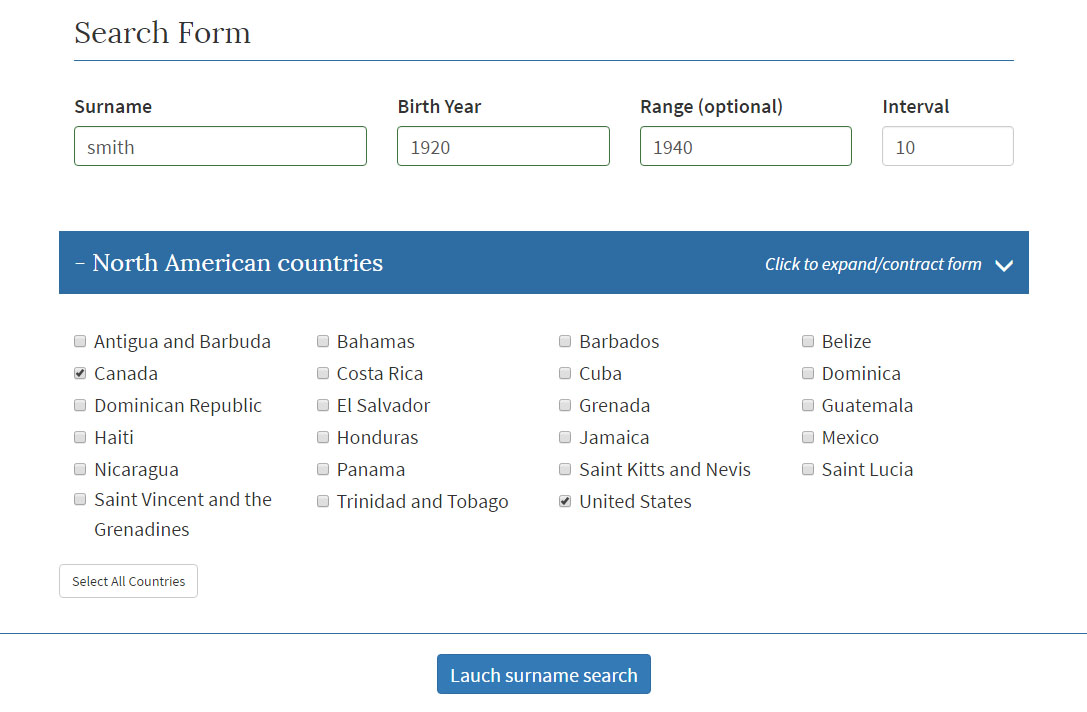
\includegraphics[width=\linewidth]{11/03_surnamesSearch/05_checkboxes}
    \centering
    \caption{Caselles de selecció creades amb Mustache}\label{fig:checkboxes}
\end{figure}
